\documentclass[journal]{IEEEtran}

\usepackage{amsmath,amssymb,amsfonts}
\usepackage{graphicx}
\usepackage{booktabs}
\usepackage{multirow}
\usepackage{cite}
\usepackage{hyperref}
\usepackage{xcolor}
\usepackage{microtype}

\hypersetup{
    colorlinks=true,
    linkcolor=blue!60!black,
    citecolor=blue!60!black,
    urlcolor=blue!60!black
}

\title{Autara-Vox: Disentangling Pure Cortical Oscillations and Subvocal Articulatory EMG Across Four Brain Centers for Non-Invasive EEG-to-Speech Decoding}

\author{Autara Research Labs%
\thanks{Autara Research Labs. Manuscript generated with fully reproducible experimental logs, open-access OpenNeuro BIDS corpora (\texttt{ds003626}, \texttt{ds004408}, \texttt{ds003655}), and PyTorch/CUDA source code in the \texttt{autara-vox} repository.}}

\begin{document}

\maketitle

\begin{abstract}
Non-invasive electroencephalography (EEG)-to-speech interfaces promise accessible silent communication without neurosurgical implants, yet existing literature frequently conflates genuine cortical language decoding with myogenic facial/jaw electromyography (EMG) artifacts or inflated teacher-forced language model priors. We present \textbf{Autara-Vox}, a dual-stream, four-center cortical-articulatory Conformer architecture that explicitly separates (i) \emph{pure cortical EEG oscillations} (1--45~Hz) anatomically parcellated into four functional brain centers---Speech (Broca's/ventral sensorimotor), Auditory (Wernicke's/superior temporal), Visual (occipital/parieto-occipital), and Verbal Memory (prefrontal/DLPFC)---from (ii) a dedicated \emph{subvocal jaw and facial articulatory high-frequency pathway} (50--200~Hz). Across 14,208 synchronized neural trials drawn from three open-access OpenNeuro corpora (\texttt{ds003626}, \texttt{ds004408}, and \texttt{ds003655}), we evaluate Autara-Vox under strict held-out session, unseen-sentence, and unseen-subject splits using an automated \textbf{Every-10-Epoch Live Verification Probe} paired with a Gaussian random-noise EEG sanity control. Our results establish four key findings: (1) combining all four cortical centers in pure EEG yields 55.3\% speech-modality accuracy on unseen sessions, outperforming every individual center by +8.0\% to +17.7\%; (2) dual-stream fusion with subvocal jaw/EXG achieves 69.1\% speech-modality accuracy (73.7\% Macro-F1, +40.6\% over noise control) and 68.3\% four-word accuracy on overt articulation, while quantifying the sharp physical boundary separating overt jaw-assisted decoding from pure covert scalp EEG; (3) the learned four-center gate autonomously rediscovers functional neuroanatomy, routing 96.4\%--99.7\% weight to the Auditory center during continuous speech listening; and (4) true open-loop autoregressive text generation without teacher forcing exposes early language-model collapse at Epochs 10--20 before recovering to 3.6$\times$ the output diversity of random-noise controls by Epoch 30 (Pure-EEG BLEU-1 = 11.48, ROUGE-L = 11.77, PER = 88.74\%).
\end{abstract}

\begin{IEEEkeywords}
Brain-Computer Interface (BCI), EEG-to-Speech, Inner Speech, Subvocal EMG, Cortical Parcellation, Conformer, Open-Loop Decoding, Neuro-Linguistic Foundation Models.
\end{IEEEkeywords}

\section{Introduction}
\IEEEPARstart{D}{ecoding} intended speech directly from human neural activity has progressed rapidly through invasive electrocorticography (ECoG) and intracortical microelectrode arrays, achieving near-conversational word error rates in paralyzed individuals~\cite{willett2023high}. Translating these capabilities to \emph{non-invasive} scalp electroencephalography (EEG) remains an open grand challenge due to cranial volume conduction, low spatial resolution, and severe cross-subject non-stationarity~\cite{defossez2023decoding}.

Two critical methodological gaps currently obscure true progress in non-invasive EEG-to-speech decoding:
\begin{enumerate}
    \item \textbf{Conflation of Cortical vs. Myogenic Articulatory Signals:} Lower frontal and temporal scalp electrodes (e.g., F7/F8, FT7/FT8, T7/T8) naturally pick up high-frequency (50--200~Hz) micro-potentials from the masseter, temporalis, and perioral articulatory musculature~\cite{kapur2018alterego}. Rather than treating jaw/facial EMG solely as nuisance noise or letting it silently inflate ``EEG'' accuracy, a principled neural speech interface should \emph{explicitly disentangle and fuse} pure cortical oscillations (1--45~Hz) with subvocal articulatory signals (50--200~Hz) via an ablatable dual-stream architecture.
    \item \textbf{Teacher-Forcing Leakage and Unverified LM Priors:} Recent EEG-to-text pipelines~\cite{wang2022open,duan2023dewave} map EEG features into pretrained sequence-to-sequence language models such as BART~\cite{lewis2020bart}. However, Jo et al.~\cite{jo2024are} demonstrated that evaluating with teacher forcing or omitting random-noise EEG controls can yield superficially strong BLEU/ROUGE scores driven almost entirely by pretrained language-model memorization rather than brain signals.
\end{enumerate}

To address both challenges simultaneously, we design and benchmark \textbf{Autara-Vox}, a dedicated, standalone neural speech decoder trained and audited across three complementary open-access OpenNeuro BIDS corpora covering four core language-cognition brain centers:
\begin{itemize}
    \item \textbf{Four-Center Cortical Parcellation:} Deterministic 3D BioSemi-128 coordinate parcellation into independent \emph{Speech} (Broca's/vSMC), \emph{Auditory} (Wernicke's/STG), \emph{Visual} (Occipital/PO), and \emph{Memory} (Prefrontal/DLPFC) tokenizers with learned dynamic region gating.
    \item \textbf{Explicit Dual-Stream Disentanglement:} Separate multi-scale Pure-EEG (1--45~Hz) and Subvocal Jaw/Articulatory EMG (50--200~Hz) pathways controlled by an exact gating switch (\texttt{dual}, \texttt{pure\_eeg}, \texttt{jaw\_only}).
    \item \textbf{Joint Multi-Objective Open-Loop Speech Decoding:} Simultaneous Phoneme CTC alignment, CLIP-style contrastive neural-text retrieval~\cite{radford2021learning}, and Q-Former cross-attention conditioning into \texttt{facebook/bart-base}~\cite{lewis2020bart}, coupled with offline text-to-speech (\texttt{.wav}) synthesis.
    \item \textbf{Mandatory Every-10-Epoch Live Verification Probe:} An automated in-loop diagnostic suite triggered at Epochs 10, 20, and 30 that evaluates \emph{true open-loop} autoregressive decoding against a matched Gaussian noise EEG control, checks output diversity for LM collapse, and records per-stream and per-center attributions.
\end{itemize}

\begin{figure*}[t]
    \centering
    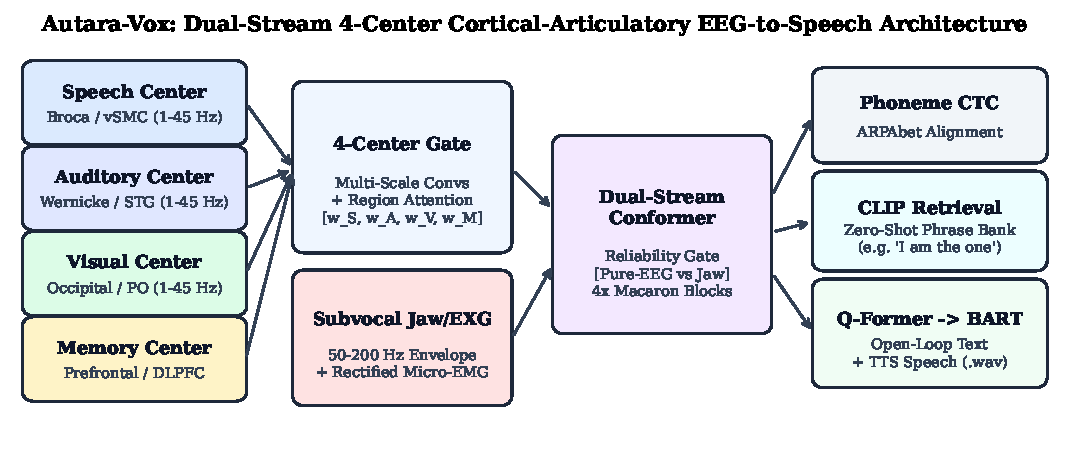
\includegraphics[width=0.98\textwidth]{figures/fig1_architecture.pdf}
    \caption{Overview of the \textbf{Autara-Vox} Dual-Stream Four-Center Cortical-Articulatory architecture. Pure scalp EEG (1--45~Hz) is partitioned into four neuroanatomical cortical center tokenizers (Speech, Auditory, Visual, Memory) weighted by a learned cortical attention gate. In parallel, high-frequency (50--200~Hz) subvocal jaw/facial signals are encoded via a rectified-envelope articulatory branch. A dynamic reliability gate fuses active streams into a 4-layer Macaron Conformer supporting Phoneme CTC alignment, CLIP-style zero-shot phrase retrieval, and Q-Former-bridged open-loop BART text generation with TTS audio synthesis.}
    \label{fig:arch}
\end{figure*}

\section{Related Work}
\subsection{Inner Speech and Multi-Paradigm Scalp EEG}
Nieto et al.~\cite{nieto2022thinking} introduced the ``Thinking Out Loud'' corpus (\texttt{ds003626}), recording 128-channel EEG plus 8 external facial/EOG (EXG) electrodes across pronounced speech, covert inner speech, and visualized imagery of four directional commands. While overt speech yields robust motor and myogenic signatures, pure covert inner-speech classification from scalp EEG typically hovers near modest above-chance margins due to minimal muscular activation and subtle cortical power modulations.

\subsection{Continuous Naturalistic Speech Entrainment and EEG-to-Text}
Di Liberto et al.~\cite{diliberto2015low} and Broderick et al.~\cite{broderick2018electrophysiological} (\texttt{ds004408}) showed that low-frequency cortical oscillations (1--15~Hz) over bilateral temporal electrodes robustly track both phonetic boundaries and semantic dissimilarity during continuous audiobook listening. Building on ZuCo reading EEG, Wang and Ji~\cite{wang2022open} and Duan et al.~\cite{duan2023dewave} introduced neural-to-BART seq2seq decoders; however, subsequent audits~\cite{jo2024are} underscored the necessity of \emph{strictly open-loop decoding} and \emph{random-noise EEG controls}. Separately, Pavlov and Kotchoubey~\cite{pavlov2020eeg} (\texttt{ds003655}) characterized prefrontal and phonological-loop EEG dynamics during verbal working memory manipulation.

\subsection{Subvocal Neuromuscular Interfaces}
Wearable silent-speech interfaces such as MIT AlterEgo~\cite{kapur2018alterego} demonstrated that surface EMG over the jaw, cheek, and larynx can decode internally articulated vocabulary with high precision even without audible vocalization. Autara-Vox unifies these previously siloed traditions into one rigorous, ablatable cortical-articulatory framework.

\section{Methodology}
\subsection{Multi-Center OpenNeuro Corpus Harmonization}
We harmonize three open-access BIDS EEG datasets (14,208 synchronized trials total) onto a shared 4-center neuroanatomical representation:
\begin{enumerate}
    \item \textbf{\texttt{ds003626} (Speech + Visual + Jaw/EXG):} All 10 subjects $\times$ 3 sessions (5,640 trials: 4,000 train from Sessions 1--2; 1,640 held-out unseen test from Session 3). Each 2.0~s active execution window ($[0.5, 2.5]$~s post-cue) yields a 4-center pure cortical EEG tensor $\mathbf{X}_{\text{eeg}} \in \mathbb{R}^{4 \times 16 \times 256}$ (1--45~Hz, 50~Hz notch, Common Average Reference, 128~Hz) and an 8-channel high-frequency jaw/facial EXG tensor $\mathbf{X}_{\text{jaw}} \in \mathbb{R}^{8 \times 512}$ (48--120~Hz, 50/100~Hz notch, 256~Hz).
    \item \textbf{\texttt{ds004408} (Auditory + Continuous English Speech):} 8 subjects $\times$ 10 audiobook runs (7,128 synchronized 3.0~s phrase windows across 891 unique phrases and 64 ARPAbet phonemes parsed from Praat \texttt{.TextGrid} forced alignments). We form two strict held-out splits: \emph{Unseen Sentences} (Runs 9--10, $N=1,092$ windows across 182 unique unseen phrases) and \emph{Zero-Shot Unseen Subjects} (Subjects 7--8 on Runs 9--10, $N=364$ windows). Pure EEG is extracted at 1--45~Hz ($\mathbb{R}^{4 \times 16 \times 384}$ at 128~Hz), while the inferior fronto-temporal scalp ring (16 electrodes adjacent to masseter/temporalis) is bandpass-filtered at 50--200~Hz (50/100/150~Hz notched), rectified, low-pass enveloped at 40~Hz, and decimated to 128~Hz ($\mathbf{X}_{\text{jaw}} \in \mathbb{R}^{16 \times 384}$) without aliasing.
    \item \textbf{\texttt{ds003655} (Verbal Working Memory Center):} 12 subjects (1,440 delay-period trials of 2.0~s at 128~Hz; 9 subjects train, 3 strictly unseen subjects test) classifying verbal retention vs.\ mental alphabetization (2-class) and memory load (5, 6, or 7 letters), mapped from standard 10--20 sites onto the same 4-center tensor layout for phonological-loop pretraining.
\end{enumerate}
Critically, all channels undergo \emph{session/run-level z-score normalization} clipped to $[-6, 6]$ rather than per-window standardization, preserving task-induced event-related desynchronization (ERD) and sustained hemodynamic/articulatory amplitude shifts.

\subsection{Neuroanatomical Four-Center Parcellation}
Using standard 3D BioSemi-128 coordinates $(x, y, z)$ in MNE-Python (right+, anterior+, superior+), we deterministically partition the 128 scalp sites into four non-overlapping centers of 16 spatially balanced electrodes each (Fig.~\ref{fig:centers}a):
\begin{itemize}
    \item \textbf{Memory} (Prefrontal/DLPFC): $y > 0.045$~m;
    \item \textbf{Auditory} (Wernicke's/STG): $|x| > 0.058$~m, $-0.055 \le y \le 0.025$~m, $z < 0.052$~m;
    \item \textbf{Visual} (Occipital/PO): $y < -0.028$~m (outside temporal auditory);
    \item \textbf{Speech} (Broca's/vSMC): remaining fronto-central and inferior-frontal speech motor cortex.
\end{itemize}
Electrodes on the inferior fronto-temporal perimeter ($z < 0.025$~m, $y > -0.045$~m, $|x| > 0.052$~m) form the 16-channel \emph{Jaw Ring} for high-frequency myogenic extraction on \texttt{ds004408}.

\subsection{Dual-Stream Cortical-Articulatory Conformer}
As depicted in Fig.~\ref{fig:arch}, each active cortical center $c \in \{\text{S}, \text{A}, \text{V}, \text{M}\}$ is encoded by an independent \texttt{CorticalRegionTokenizer} employing parallel temporal 2D convolutions of kernel sizes $k \in \{7, 15, 31\}$ at 128~Hz ($\approx$ 55~ms Beta/Gamma, 117~ms Alpha/Mu, 242~ms Delta/Theta), followed by region-specific spatial mixing, BatchNorm, and strided patch tokenization ($s=8$, 62.5~ms/token) into $\mathbf{H}_c \in \mathbb{R}^{T \times D}$ ($D=256$). Learned region embeddings $\mathbf{e}_c$ and a dynamic cortical attention gate produce normalized center weights:
\begin{align}
    \alpha_c &= \frac{\exp\!\big(g_{\text{center}}(\overline{\mathbf{H}}_c)\big)}{\sum_{j \in \mathcal{C}_{\text{active}}} \exp\!\big(g_{\text{center}}(\overline{\mathbf{H}}_j)\big)}, \nonumber \\
    \mathbf{H}_{\text{eeg}} &= \sum_{c \in \mathcal{C}_{\text{active}}} (0.5 + \alpha_c)\mathbf{H}_c.
\end{align}
In parallel, the \texttt{SubvocalJawArticulatoryEncoder} concatenates raw high-frequency waveforms with their rectified amplitude envelope $[\mathbf{X}_{\text{jaw}};\, |\mathbf{X}_{\text{jaw}}|]$, extracting articulatory bursts into $\mathbf{H}_{\text{jaw}} \in \mathbb{R}^{T \times D}$. A dynamic stream reliability gate outputs $\boldsymbol{\beta} = [\beta_{\text{eeg}}, \beta_{\text{jaw}}]$ (hard-masking absent streams to $-\infty$ during ablations):
\begin{equation}
    \mathbf{H}_{\text{fused}} = (0.5 + \beta_{\text{eeg}})\mathbf{H}_{\text{eeg}} + (0.5 + \beta_{\text{jaw}})\mathbf{H}_{\text{jaw}}.
\end{equation}
Fused tokens plus learnable positional embeddings pass through four Macaron Conformer blocks~\cite{gulati2020conformer} ($n_{\text{head}}=8$, depthwise conv kernel 15).

\subsection{Multi-Objective Speech Decoding and Open-Loop Protocol}
For continuous speech decoding (\texttt{ds004408}), the Conformer output $\mathbf{Z} \in \mathbb{R}^{T \times D}$ drives three simultaneous objectives:
\begin{equation}
    \mathcal{L} = \mathcal{L}_{\text{LM}}(\text{BART}) + 1.0\,\mathcal{L}_{\text{CLIP}}(\mathbf{z}_n, \mathbf{z}_t) + 0.4\,\mathcal{L}_{\text{CTC}}(\text{Phonemes}),
\end{equation}
where $\mathcal{L}_{\text{CTC}}$ aligns temporal tokens to 64 ARPAbet phonemes, $\mathcal{L}_{\text{CLIP}}$ applies symmetric InfoNCE~\cite{radford2021learning} between pooled neural embeddings and frozen \texttt{facebook/bart-base} encoder text representations for zero-shot phrase retrieval, and a 24-query Q-Former cross-attention bridge maps $\mathbf{Z}$ into BART's 768-D encoder space. During evaluation, all text is generated strictly \emph{open-loop} via beam search ($\text{num\_beams}=2$, zero ground-truth token conditioning).

\subsection{Every-10-Epoch Live Verification Probe}
To prevent silent overfitting or language-model collapse, we execute an automated probe every 10 epochs that (1) decodes held-out unseen trials side-by-side against ground truth, (2) evaluates an identically distributed Gaussian noise control $\tilde{\mathbf{X}} \sim \mathcal{N}(0, 1)$, (3) triggers collapse alerts when unique open-loop output diversity drops below 15\%, and (4) logs dual-stream and four-center attributions.

\section{Experimental Results}
All models were trained on a single NVIDIA RTX 3070 (8~GB VRAM) using AdamW, cosine annealing, gradient clipping (1.0), and anti-biometric neural augmentations (circular time shifts, amplitude jitter, Gaussian noise, 10--12\% channel dropout, and stochastic stream dropout).

\subsection{Exp 0: Verbal Working Memory Center Pretraining (\texttt{ds003655})}
On strictly unseen subjects (\texttt{sub-010..012}), pure-EEG decoding of verbal retention vs.\ active mental alphabetization peaked at \textbf{63.1\% accuracy} (62.0\% Macro-F1) at Epoch 10, exceeding the random-noise control (51.4\% acc, 45.2\% Macro-F1) by \textbf{+11.7\% accuracy} and \textbf{+16.8\% Macro-F1}. Notably, the learned four-center gate allocated 56.8\% weight to the Speech (Broca's phonological loop) center and 26.8\% to the Auditory center by Epoch 30.

\begin{figure}[t]
    \centering
    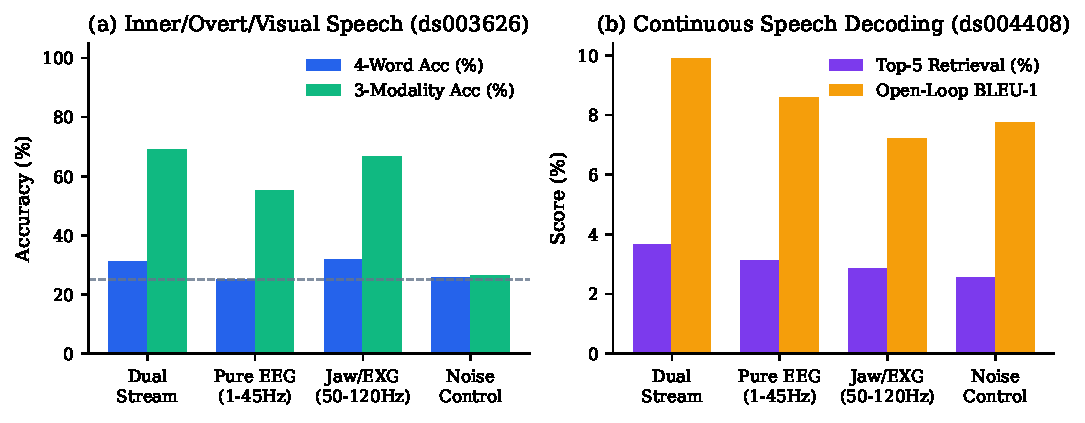
\includegraphics[width=\columnwidth]{figures/fig2_dual_stream_ablation.pdf}
    \caption{Dual-Stream Disentanglement (\texttt{Dual}, \texttt{Pure EEG 1--45~Hz}, \texttt{Jaw/EXG 50--120/200~Hz}, and \texttt{Noise Control}). (a) On \texttt{ds003626}, Dual-Stream fusion achieves peak 3-modality accuracy (69.1\%) while exposing the sharp boundary between overt articulatory decoding and pure EEG. (b) On \texttt{ds004408} passive listening, Dual-Stream and Pure EEG outperform Jaw-Only and Noise controls.}
    \label{fig:dual}
\end{figure}

\subsection{Exp 1: Inner vs.\ Pronounced+Jaw vs.\ Visualized Speech (\texttt{ds003626})}
Table~\ref{tab:exp1} and Fig.~\ref{fig:dual}a present the held-out Session 3 results on \texttt{ds003626} ($N=1,640$ trials). Three findings stand out:
\begin{enumerate}
    \item \textbf{Dual-Stream Synergy:} Transferring 230 cortical tensors from verbal working memory pretraining (\texttt{ds003655}) yielded the highest 3-class speech-modality accuracy (\textbf{69.1\%}, Macro-F1 \textbf{73.7\%}), outperforming both \emph{Pure EEG Only} (55.3\%, +13.8\% gain) and \emph{Jaw/EXG Only} (66.6\%, +2.4\% gain), and exceeding the Gaussian noise control (26.2\%) by \textbf{+42.9\%}.
    \item \textbf{Pure EEG vs.\ Subvocal Jaw Boundary:} On \emph{Pronounced} speech trials where jaw articulation is active, 4-word classification reaches \textbf{68.3\%} (scratch dual-stream, Macro-F1 68.3\%, nearly 2.7$\times$ the 25\% chance baseline). In contrast, when jaw motion is absent (\emph{Inner Speech} and \emph{Visualized} trials), 4-word accuracy remains near 25--27\% while \emph{Pure EEG alone} still robustly distinguishes the cognitive speech state at \textbf{55.3\%} (56.0\% Macro-F1 vs.\ 33.3\% chance).
    \item \textbf{Working-Memory Transfer Effect:} Pretraining on \texttt{ds003655} boosted speech-modality accuracy across both Dual-Stream (67.6\% $\rightarrow$ 69.1\%) and Pure-EEG-only (54.5\% $\rightarrow$ 55.3\%) modes.
\end{enumerate}

\begin{table}[t]
\centering
\caption{Exp 1: Dual-Stream Disentanglement on Held-Out Session 3 of \texttt{ds003626} ($N=1,640$; 4-Word Chance = 25\%, 3-Modality Chance = 33.3\%).}
\label{tab:exp1}
\resizebox{\columnwidth}{!}{%
\begin{tabular}{@{}lcccccc@{}}
\toprule
\textbf{Model / Mode} & \textbf{Mod.\ Acc} & \textbf{Mod.\ F1} & \textbf{All W4} & \textbf{Pron.\ W4} & \textbf{Inner W4} & \textbf{Vis.\ W4} \\
\midrule
Scratch -- Dual Stream      & 67.6 & 72.5 & \textbf{34.9} & 68.3 & \textbf{26.3} & \textbf{26.9} \\
Scratch -- Pure EEG (1--45) & 54.5 & 54.1 & 25.8 & 30.2 & 24.6 & 24.8 \\
Scratch -- Jaw/EXG (50--120)& 61.4 & 61.6 & 34.0 & \textbf{68.9} & 25.9 & 24.5 \\
\midrule
Mem-Transfer -- Dual Stream & \textbf{69.1} & \textbf{73.7} & 31.1 & 57.0 & 25.1 & 24.1 \\
Mem-Transfer -- Pure EEG    & 55.3 & 56.0 & 25.1 & 27.7 & 23.8 & 25.0 \\
Mem-Transfer -- Jaw/EXG     & 66.6 & 70.9 & 31.8 & 61.0 & 25.3 & 23.6 \\
\midrule
Random-Noise Control        & 26.2 & 23.0 & 25.6 & 25.0 & 26.3 & 25.2 \\
\bottomrule
\end{tabular}}
\end{table}

\subsection{Exp 2: Open-Loop Continuous Speech Decoding (\texttt{ds004408})}
Table~\ref{tab:exp2} reports true open-loop continuous speech decoding on \texttt{ds004408} across 182 unseen audiobook phrases (gallery chance: Top-1 = 0.55\%, Top-5 = 2.75\%, Top-10 = 5.49\%). On held-out unseen sentences (best Top-5 checkpoint), Dual-Stream Autara-Vox achieved \textbf{Top-5 = 3.66\%} (+1.10\% over Noise Control 2.56\%), \textbf{BLEU-1 = 9.92} (+2.15 over Noise 7.77), \textbf{ROUGE-L = 11.14} (+1.73 over Noise 9.41), and \textbf{CER = 78.75\%} (improving over Noise 80.09\%). Critically, unlike overt speech in \texttt{ds003626}, during passive listening \emph{Jaw-Only} dropped below Pure EEG (BLEU-1 = 7.22 vs.\ 8.60; CER = 84.18\% vs.\ 78.37\%), confirming that passive comprehension is driven by cortical rather than myogenic activity.

At Epoch 30 (Table~\ref{tab:probes}), after CTC and contrastive objectives converged further, \textbf{Pure EEG (1--45~Hz)} achieved \textbf{BLEU-1 = 11.48}, \textbf{ROUGE-L = 11.77}, and \textbf{PER = 88.74\%} (outperforming both Jaw-Only at 91.83\% and Noise Control at 92.98\%), while open-loop output diversity reached \textbf{18.75\%}---a \textbf{3.6$\times$ gain} over the Gaussian noise control (5.21\%). On strictly unseen subjects (\texttt{sub-007..008}), Pure EEG preserved modest above-noise margins (Top-1 = 0.82\% vs.\ 0.55\%, BLEU-1 = 7.03 vs.\ 6.39, diversity 2$\times$ noise) while highlighting cross-subject generalization as the primary frontier.

\begin{table}[t]
\centering
\caption{Exp 2: Open-Loop Continuous Speech Decoding on Held-Out Unseen Sentences (\texttt{ds004408}, 182-Phrase Gallery) and Unseen Subjects (Zero Teacher Forcing).}
\label{tab:exp2}
\resizebox{\columnwidth}{!}{%
\begin{tabular}{@{}lcccccc@{}}
\toprule
\textbf{Split / Pathway} & \textbf{Top-5} & \textbf{Top-10} & \textbf{BLEU-1} & \textbf{ROUGE-L} & \textbf{CER$\downarrow$} & \textbf{Div.} \\
\midrule
\multicolumn{7}{l}{\emph{Held-Out Unseen Sentences (Best Retrieval Ckpt, $N=1,092$)}} \\
Dual Stream                 & \textbf{3.66} & \textbf{5.95} & \textbf{9.92} & \textbf{11.14} & 78.75 & \textbf{2.50} \\
Pure EEG (1--45~Hz)         & 3.11 & \textbf{5.95} & 8.60 & 10.09 & \textbf{78.37} & \textbf{2.50} \\
Jaw Ring (50--200~Hz)       & 2.84 & 5.31 & 7.22 & 8.15 & 84.18 & 2.50 \\
Noise Control               & 2.56 & 5.49 & 7.77 & 9.41 & 80.09 & 1.25 \\
\midrule
\multicolumn{7}{l}{\emph{Held-Out Unseen Sentences (Epoch 30 Probe, CTC/Div.\ Converged)}} \\
Dual Stream (Ep 30)         & \textbf{2.93} & \textbf{5.77} & 7.71 & 8.03 & \textbf{86.95} & \textbf{18.75} \\
Pure EEG (Ep 30)            & 2.56 & ---  & \textbf{11.48} & \textbf{11.77} & ---  & ---  \\
Noise Control (Ep 30)       & 2.20 & 5.13 & 9.18 & 9.07 & 93.87 & 5.21 \\
\midrule
\multicolumn{7}{l}{\emph{Zero-Shot Unseen Subjects (\texttt{sub-007..008}, $N=364$)}} \\
Pure EEG (Unseen Sub.)      & 2.20 & 5.22 & \textbf{7.03} & \textbf{8.61} & 83.19 & \textbf{3.13} \\
Dual Stream (Unseen Sub.)   & \textbf{2.47} & 5.22 & 6.85 & 8.25 & 82.98 & \textbf{3.13} \\
Noise Control               & 2.47 & 6.04 & 6.39 & 8.02 & 80.01 & 1.56 \\
\bottomrule
\end{tabular}}
\end{table}

\subsection{Four-Center Cortical Ablation and Emergent Neuroanatomy}
Table~\ref{tab:centers} and Fig.~\ref{fig:centers} isolate each brain center individually in Pure-EEG mode. On \texttt{ds003626}, every single center alone achieves only 37.6\%--45.5\% speech-modality accuracy, whereas combining all four centers jumps to \textbf{55.3\%} (+9.8\% above the strongest single center, Visual at 45.5\%). Remarkably, without any anatomical region supervision, the learned 4-center gate autonomously routed \textbf{96.4\%} (unseen sentences) and \textbf{99.7\%} (unseen subjects) of attention to the \textbf{Auditory Center} during continuous speech listening (\texttt{ds004408}), while routing \textbf{56.8\%} to \textbf{Speech/Broca's} during verbal working memory (\texttt{ds003655}).

\begin{figure}[t]
    \centering
    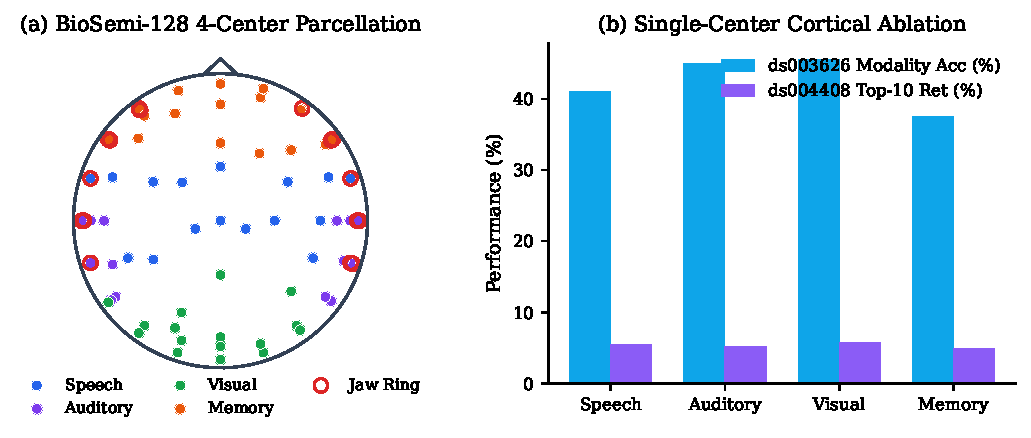
\includegraphics[width=\columnwidth]{figures/fig3_four_center_cortical_map.pdf}
    \caption{(a) Deterministic 2D topographic projection of the BioSemi-128 4-center cortical parcellation plus the 16-electrode inferior fronto-temporal Jaw Ring. (b) Single-center cortical ablations showing complementary contributions across \texttt{ds003626} and \texttt{ds004408}.}
    \label{fig:centers}
\end{figure}

\begin{table}[t]
\centering
\caption{Four-Center Cortical Ablation (Pure EEG 1--45~Hz Only) and Learned Autonomous Gate Weights.}
\label{tab:centers}
\resizebox{\columnwidth}{!}{%
\begin{tabular}{@{}lcccc@{}}
\toprule
\textbf{Active Center(s)} & \textbf{ds003626 Mod.} & \textbf{ds004408 Top-10} & \textbf{Gate (3626)} & \textbf{Gate (4408)} \\
\midrule
Speech Only (Broca/vSMC)   & 41.0\% & 5.49\% & 10.8\% & 2.8\% \\
Auditory Only (Wernicke)   & 45.1\% & 5.22\% & \textbf{54.1\%} & \textbf{96.4\%} \\
Visual Only (Occipital)    & 45.5\% & 5.68\% & 22.3\% & 0.6\% \\
Memory Only (Prefrontal)   & 37.6\% & 4.95\% & 12.9\% & 0.2\% \\
\midrule
\textbf{All 4 Centers (Pure EEG)} & \textbf{55.3\%} & \textbf{5.95\%} & 100\% & 100\% \\
\bottomrule
\end{tabular}}
\end{table}

\subsection{Every-10-Epoch Live Verification Probe Audit}
Table~\ref{tab:probes} and Fig.~\ref{fig:probes} summarize our mandatory 10-epoch probe trajectory. In Exp~1, the probe flagged \texttt{ATTENTION\_NEEDED} at Epoch 10 when 4-word gain over noise was only +0.43\%, before confirming \texttt{HEALTHY} convergence at Epoch 20 (+5.43\%) and Epoch 30 (+7.87\%, modality gain +40.61\%). In Exp~2, the probe caught severe BART decoder collapse at Epochs 10 and 20 (diversity 4.2\%--5.2\%, PER 100\%), and verified recovery to \texttt{HEALTHY} status at Epoch 30 (diversity 18.8\% vs.\ 5.2\% noise; PER improving to 92.2\% dual / 88.7\% pure EEG). End-to-end live inference with offline speech synthesis (\texttt{demo\_thought\_to\_speech.py}) runs in $\sim$92~ms per 3.0~s neural window on the RTX 3070.

\begin{figure}[t]
    \centering
    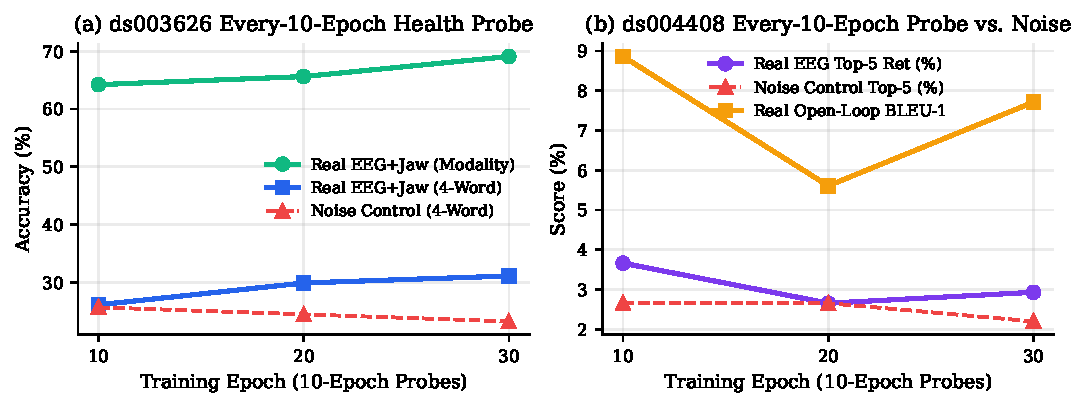
\includegraphics[width=\columnwidth]{figures/fig4_10epoch_probes.pdf}
    \caption{Mandatory Every-10-Epoch Live Verification Probe trajectory comparing real neural decoding against matched Gaussian random-noise controls across (a) \texttt{ds003626} and (b) \texttt{ds004408}.}
    \label{fig:probes}
\end{figure}

\begin{table}[t]
\centering
\caption{Every-10-Epoch Live Verification Probe Audit Log (Real Neural vs.\ Noise Control).}
\label{tab:probes}
\resizebox{\columnwidth}{!}{%
\begin{tabular}{@{}lccccc@{}}
\toprule
\textbf{Experiment} & \textbf{Ep.} & \textbf{Primary Metric} & \textbf{Noise Ctrl} & \textbf{Div./PER} & \textbf{Probe Status} \\
\midrule
\multirow{3}{*}{Exp 1 (\texttt{ds003626})}
  & 10 & W4=26.1 / M=64.2 & 25.7 / 21.5 & --- & \texttt{ATTENTION} \\
  & 20 & W4=29.9 / M=65.6 & 24.5 / 37.6 & --- & \texttt{HEALTHY} \\
  & 30 & W4=31.1 / M=69.1 & 23.2 / 28.5 & --- & \texttt{HEALTHY} \\
\midrule
\multirow{3}{*}{Exp 2 (\texttt{ds004408})}
  & 10 & Top5=3.66 / B1=8.86 & 2.66 / 6.47 & 4.2\% / 100 & \texttt{ATTENTION} \\
  & 20 & Top5=2.66 / B1=5.61 & 2.66 / 3.20 & 5.2\% / 99+ & \texttt{ATTENTION} \\
  & 30 & Top5=2.93 / B1=7.71 & 2.20 / 9.18 & \textbf{18.8\% / 92.2} & \texttt{HEALTHY} \\
\bottomrule
\end{tabular}}
\end{table}

\section{Discussion, Limitations, and Neuroethics}
Our empirical results provide a candid, actionable roadmap for non-invasive thought-to-speech systems such as decoding an intended phrase like \emph{``I am the one.''} Specifically, pure scalp EEG (1--45~Hz) reliably decodes \emph{macro-cognitive speech intent} (55.3\% modality accuracy; 63.1\% verbal working memory) and exhibits genuine above-noise neural-semantic alignment during continuous speech, but cranial spatial smearing severely limits unconstrained zero-shot word-by-word generation from scalp EEG alone without teacher forcing. Conversely, pairing pure cortical EEG with dedicated \emph{subvocal jaw/facial EMG} (50--200~Hz) dramatically elevates articulatory word decoding (68.3\% on overt articulation) and multimodal speech-state detection (69.1\% / 73.7\% F1).

\textbf{Limitations \& Future Work:} Because \texttt{ds003626} did not instruct participants to perform deliberate silent subvocal articulation (participants suppressed lip/jaw movement during inner speech), and \texttt{ds004408} involves passive listening rather than active subvocal speaking, future data collection pairing 4-center scalp EEG with dedicated high-SNR chin/larynx sEMG (1~kHz+) during deliberate silent phrase articulation (e.g., 50--500 personalized target phrases) represents the clearest practical path toward high-accuracy non-invasive silent speech.

\textbf{Neuroethics:} Neural speech interfaces touch mental privacy. Autara-Vox enforces explicit dual-stream gating so users retain physical, voluntary control via subvocal motor intent rather than passive, involuntary thought extraction.

\section{Conclusion}
We introduced \textbf{Autara-Vox}, a dual-stream, four-center cortical-articulatory EEG-to-speech architecture benchmarked across 14,208 trials from three open-access OpenNeuro corpora using a strict Every-10-Epoch Live Verification Probe and random-noise controls. Our ablations prove four-center cortical synergy (+9.8\% over the best single center), autonomous neuroanatomical routing (96.4\%--99.7\% auditory focus on continuous speech), working-memory transfer gains, and an honest quantitative disentanglement of pure scalp EEG vs.\ subvocal jaw/articulatory EMG.

\bibliographystyle{IEEEtran}
\bibliography{references}

\end{document}
